\section{Unmanned Aerial Systems}
Generically, an Autonomous Air System is composed of the aground ground station (GS), a communications system and an aerial element. The operation of the system is based on the fact that an operator at the ground control station directs a Datalink the operation of the aircraft based on the information that it transmits to through its sensors. Depending on the performance characteristics of the aircraft such as the ceiling in service, speed, scope, the payment burden of the same, the coverage and transmission capacity of the link data and autonomy, in the sense of decision-making capacity of the UAV, the System operation varies.\cite{Duran}
\begin{figure}[H]
\centering
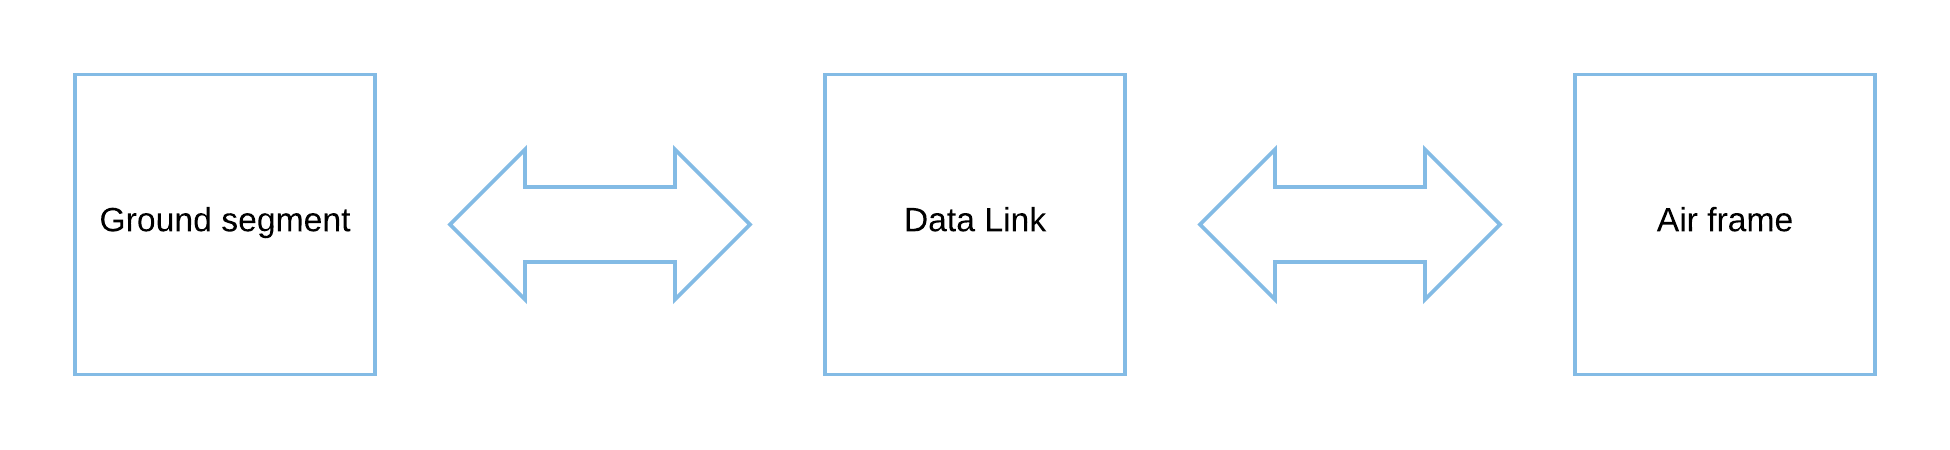
\includegraphics[width=10cm,height=10cm,keepaspectratio]{imagenes/UAS_Components.png}
\caption{UAS Block diagram}
\label{fig:block diagram}
\end{figure}

\subsection{UAS components}
As describes before there are three main components to a UAS: Ground Control Station (GCS), Data Link and Airframe. This section presents a description of each component 
\subsubsection{Ground segment} 
The ground control station is where an operator interacts with a UAS. It generally consists of several parts, usually providing feedback about UAV activity, allowing command and control of the aircraft and giving a method of override control for the system.
The GCS can be divided into the following components:
\begin{itemize}
    \item \textbf{Ground Computer:} It the computer or system where the ground station software is executed, also where the downlink of the data link is received.
    \item \textbf{Ground software:} Just as important as the software running onboard the main autopilot board in the air, is the corresponding software on the GCS, providing the human interface for configuration, monitoring, and control of the UAS. The ground software should provide:
    \begin{itemize}
        \item Compilation tools to produce the airborne software from the configurations and source code.
        \item GUI to control and interact with the UAV(s) during flight as well as mission planning and simulation.
        \item Basic simulator to ease the development of flight plans and verify some airborne code behavior.
        \item Data logging system with plot-based viewer for real-time and post-flight analysis.
        \item Number of utilities for communicating with the UAV and other agents
        \item Number of tools for calibration, etc.
        \item Control panel GUI for configuration and program management.
        \item Easy method of extending functionality with the Ivy Bus.
    \end{itemize}
    \item \text{Groundside Datalink:} offers possibilities to supervise the UAV flight from the ground. The default one uses a bidirectional wireless modem which supports both telemetry (downlink) and tele control (uplink). Thanks to this data link, flight parameters are available in real time, and full control of the navigation and tuning of one or several aircraft is possible from the ground station. The ground side of the link usually consists of a matching radio modem, like an XBee, connected to the ground station computer over USB or serial port.
    \item \text{Groundside Safelink:} The ground side of the safety link usually consists of a radio control transmitter (and safety pilot). It is used to provide manual control of the aircraft.
\end{itemize}
\subsubsection{Data link}
UAS data link is a system of monitoring-control and information transmission. Generally, it consists of the link protocol, the transport channel and the message protocol. It is designed to achieve real-time information exchange between the sensors, GCS and the UAV as well as to handle the information from flying scene situation, command control, and mission control.\cite{6305636} The data link can be divided into two: \textit{Uplink} and \textit{Downlink}:

\begin{itemize}
    \item \textbf{Donwlink:}  is used to transmit the information from the UAV to the GCS, including status data, sensor data, and graphics image data. In general, the UAV is controlled mainly through the onboard autopilot, with the GCS being used in monitoring the flight status and handling an emergency. \cite{6305636}
    \item \textbf{Uplinks:} is used to transmit the control information from the GCS to the UAV, such as flight parameters, waypoints information, and command instruction. \cite{6305636}
\end{itemize}

The UAS transmission channel consists of two parts: the data terminal equipment (DTE) and the wireless channel. DTE, composed by modem, network controllers and cryptographic equipment, is the fundamental but essential unit of the data link. The operating frequencies of data link are usually in HF, VHF, UHF, L, S, C, and K band, and the choice of frequency depends on its entrusted mission and technology system.\cite{6305636}

The radio modem is the most common DTE in the small civilian UAS. It embodies the function of radio transmission, digital modulation and error correction, provides a serial transmission with the rate between 9600bps and 19200bps, as well as supports half-duplex or full-duplex communication.\cite{6305636}

There is a third data link in a UAS system called \textit{Safe Link}. A traditional radio control transmitter and receiver pair are used to provide a manual control option for the UAV. The airborne hardware and software support the connection to a standard radio-control receiver. The autopilot reads the output from the R/C receiver on board the aircraft and decides what control mode is desired. When in manual mode, a safety pilot on the ground may use the R/C transmitter to control the aircraft. The fly-by-wire mode provides a reliable method of providing override control even though the autopilot always remains inline between R/C receiver and actuators.\cite{Hattenberger2014UsingTP}

\subsubsection{Airbone segment}
The airborne segment is the aircraft (UAV), its hardware parts including payload and all the embedded software to control the flight (from stabilization to decision making). The key components are:
\begin{itemize}
    \item Autopilot board.
    \item Altitude sensor.
    \item Inertial Measurement Unit (IMU).
    \item GPS Receiver.
    \item Datalink Radio Modem.
    \item RC receiver.
    \item Servos.
    \item Propulsion system.
    \item Batteries.
    \item Payload.
\end{itemize}
For these project, the most relevant components are Autopilot, payload and propulsion system.
\begin{figure}[H]
\centering
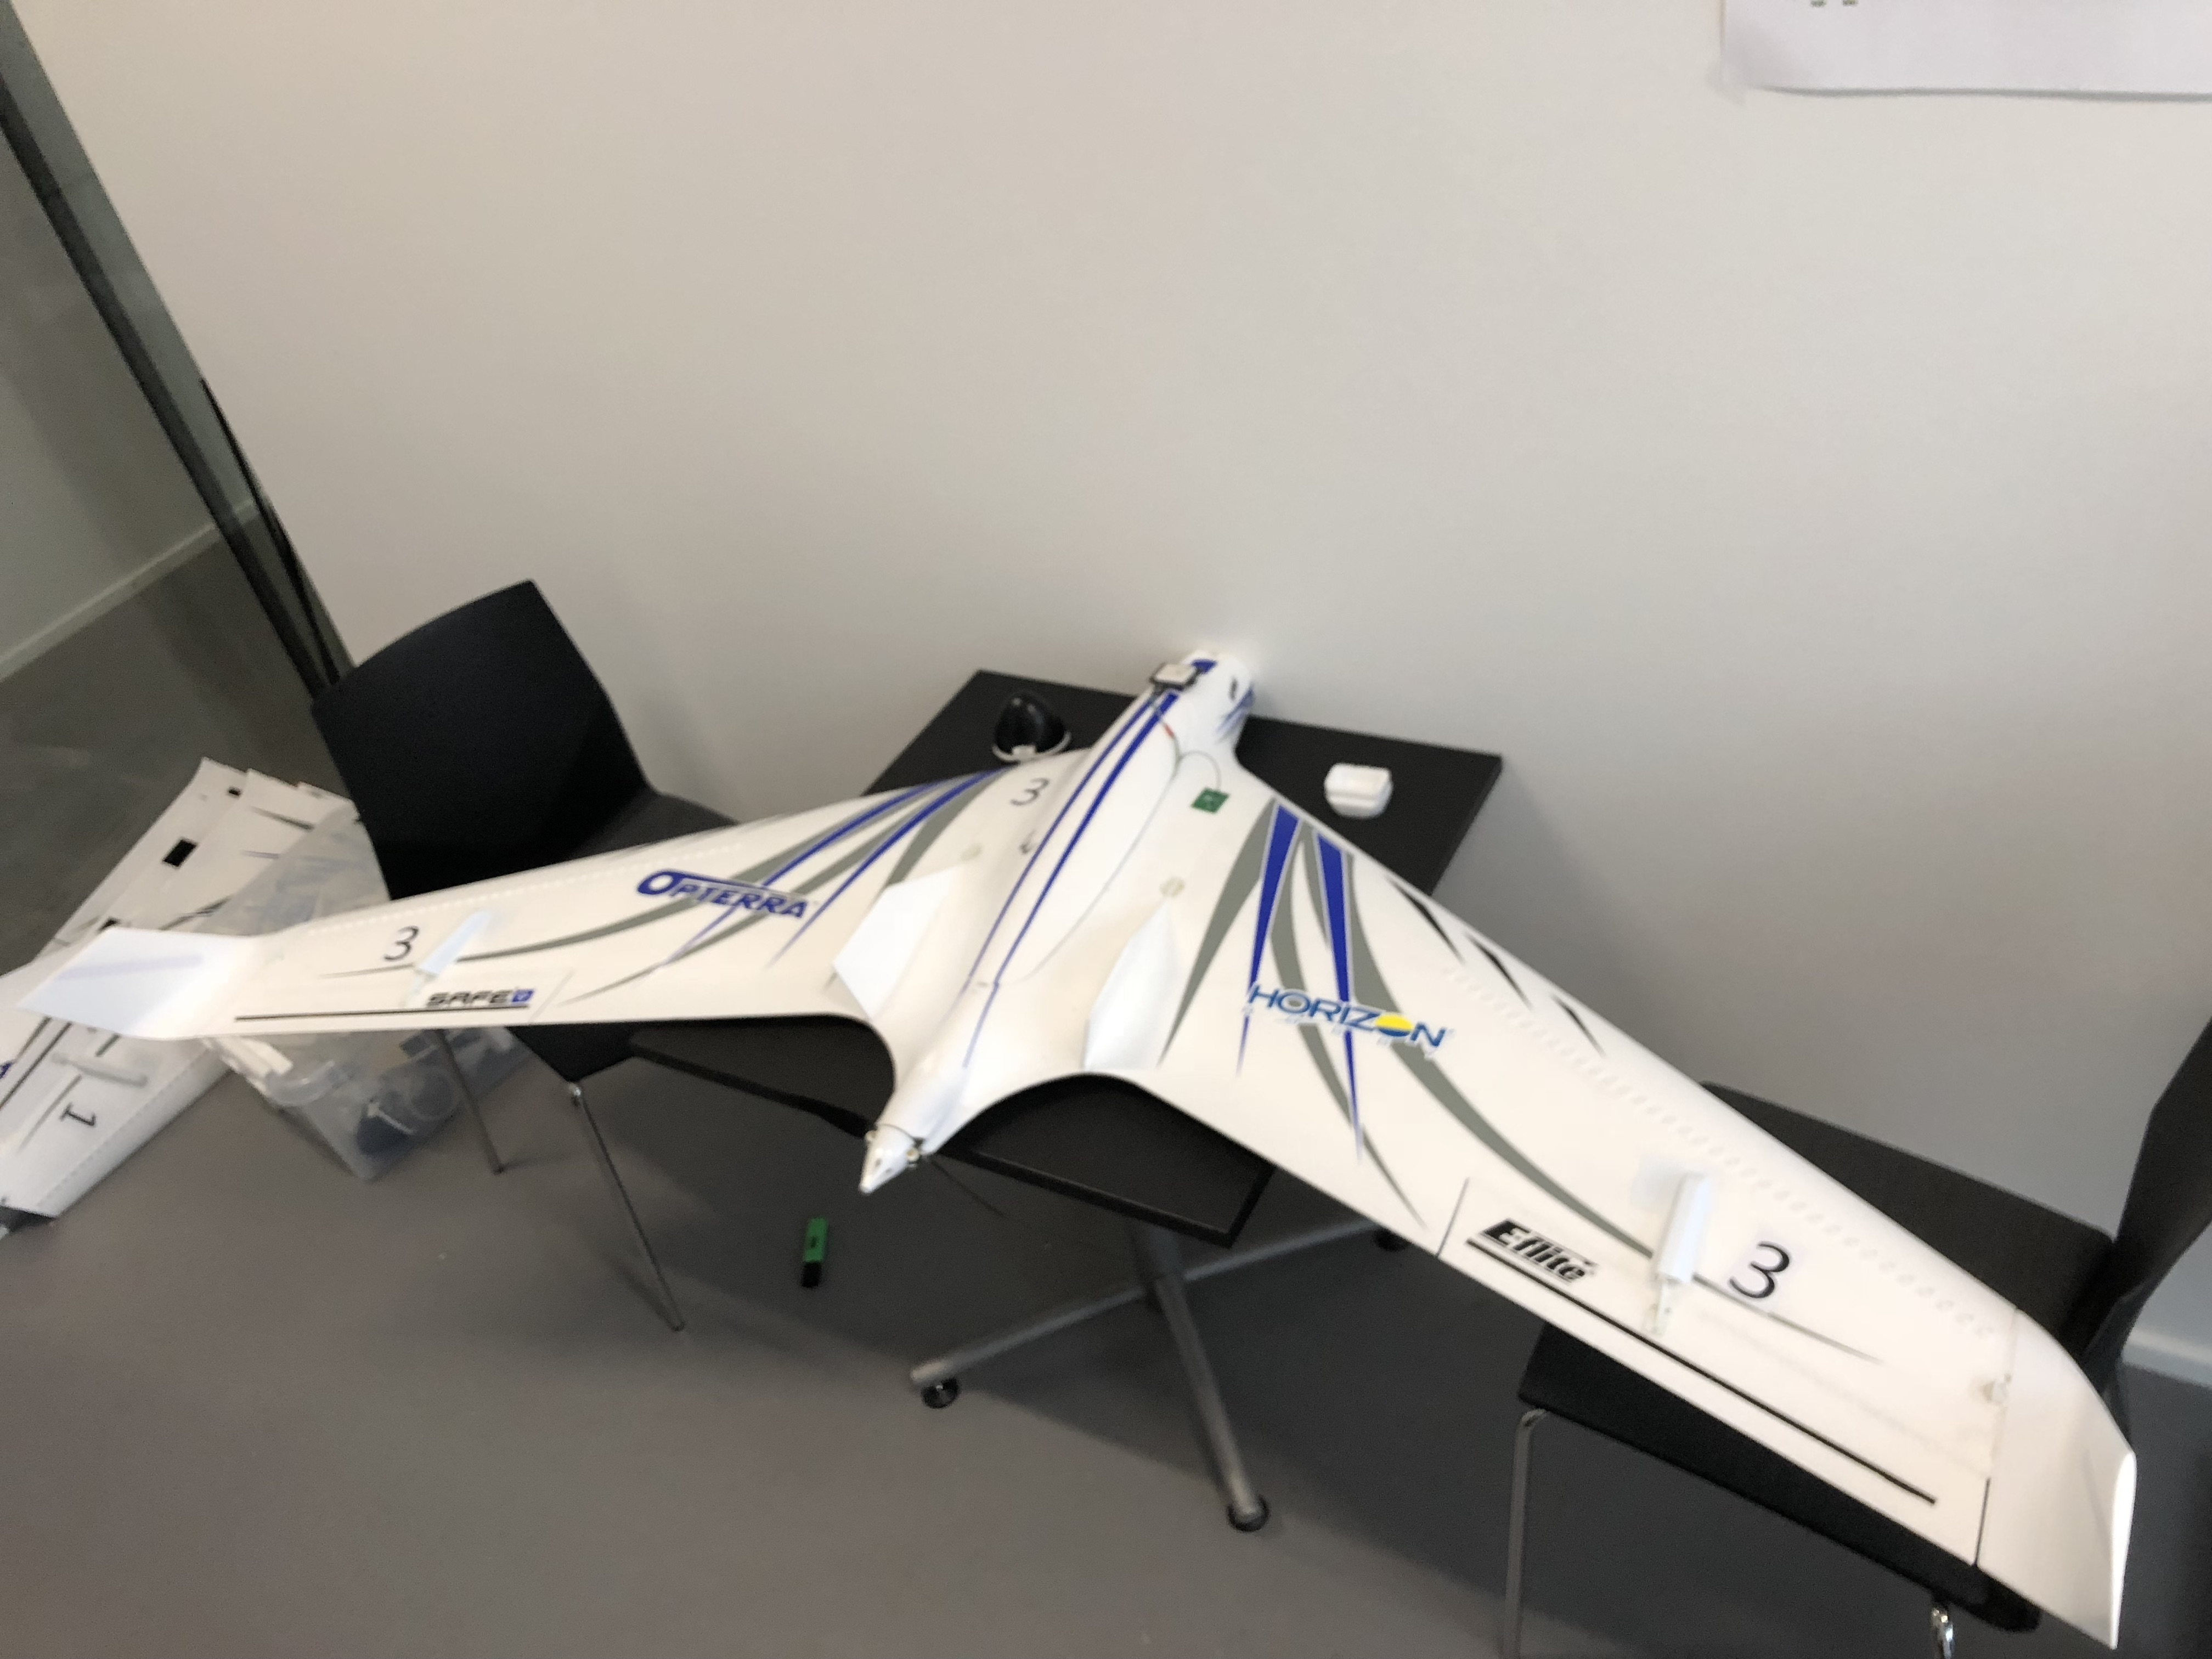
\includegraphics[width=10cm,height=10cm,keepaspectratio]{imagenes/opterra.jpg}
\caption{Opterra fixed-wing aircraft}
\label{fig:Optera}
\end{figure}
\textbf{ Autopilot} or controller board is the system responsible for carrying out all the tasks on the aircraft for the control of the UAV, it can be said that it is the brain of the platform. Its main functions are: Control the propulsion system and the stability of the UAV, manage communication with the control station and execute the instructions of the pilot. The CPU works with other modules for flight management. Collects information from a series of MEMS sensors (Micro-Electromechanical Systems) and receivers of satellite navigation, to estimate the position and orientation of the UAV system. Also establishes a communication link with the control station through a module of radio frequency.\cite{Edgar}

The autopilot, in conjunction with the other blocks, must have the ability to:
\begin{itemize}
    \item Measure and estimate the orientation and spatial location of the system.
    \item Ability to generate control signals to the actuators during the flight.
    \item Control and monitoring of the flight route.
    \item Monitoring and sending of the conditions of the system through the communication link.
    \item Control of pilot instructions on the ground.
    \item Operate sensors.
\end{itemize}

The project utilizes the apogee autopilot. Apogee is the latest in French Engineering and design from E.N.A.C.  This controller uses the latest STM32F4 processor to create a comprehensive autopilot controller board  When you add the incredibly powerful and robust software such as paparazzi.\cite{apogee}
\begin{figure}[H]
\centering
\includegraphics[width=10cm,height=10cm,keepaspectratio]{imagenes/apogee.jpg}
\caption{Apogee autopilot}
\label{fig:apogee}
\end{figure}
As mention before one of the main task performed by the autopilot is Control and monitoring of the flight route. The guidance, navigation, and control of the plane are implemented utilizing the \textit{Guiding Vector Field (GVF)} algorithm. 

The vector field algorithms are widely used in many applications of robotics, such as path-planning, obstacle avoidance, and extremum seeking. The main idea is to design a potential vector field, whose integral lines converge to the desired path. In particular, the general description of the vector field for the path following.\cite{GVF}

Guidance vector field approach, which originates in potential field method, provides an efficient and convenient way for the path following problem. It assigns a desired path angle for each point in the space. This desired path angle is usually a function of the coordinates of the corresponding point. Moreover, a series of these desired path angles determine the desired trajectory, and by tracking this trajectory, the path following objective can be finally achieved.\cite{7170894}

For fixed-wings, the output of the algorithm can be directly expressed in terms of the bank angle of the UAV to achieve coordinated turns. Furthermore, the algorithm can be tuned offline such that the physical constraints of the UAV, e.g., the maximum bank angle, does not violate in a neighborhood of the desired trajectory.\cite{7942030}

\textbf{Payload} Virtually all kinds of payloads can be attached to the airframe, the only restrictions are usually the weight and size of payloads. Most airframes are equipped with cameras. For these project, the payload is a camera pointed downwards, placed on the "belly" of the plane. 

The UAV can be categorized by different criteria: 
\begin{itemize}
    \item \textbf{Propultion type.}
    \item  \textbf{Maximum take-off weight.}
\end{itemize}
\textbf{Propulsion type} can be divided into two main categories:
\begin{itemize}
\item Fixed-wing UAS: Fixed wing UAS are characterized to have an elementary structure, aerodynamically efficient, that allows to reach high speeds and have a higher efficiency than multirotor platforms, due to the lower power consumption. The landing and take-off procedure present a difficulty to these types of UAS due to the necessity of a runway.
\item Rotatory wing: They are composed of 2 or more rotor. Its main characteristics are the ability to perform vertical take-off and landings, in addition to having a great maneuverability and flight precision. Its main disadvantage is due to its more complex electronics structure, sacrifice flight autonomy.\cite{Luis_Fernadno}
\end{itemize}

\textbf{Maximum take-off Weight}: The first classification to be established for UAS is based on the vehicle size. According to these criteria, they are a brought number of platforms that can be categorized as mini, micro, small or large dimension. Maximum Take-Off Weight (MTOW) is the parameter used to classify the UAS. MTOW is the sum of aircraft weight, maximum payload, and fuel.\cite{ICAO}


